\documentclass[conference]{IEEEtran}
\usepackage{tikz}
\usetikzlibrary{positioning, shapes.geometric, arrows.meta, fit, calc}

\begin{document}

\begin{figure}[!t]
\centering
\scriptsize
\resizebox{\columnwidth}{!}{%
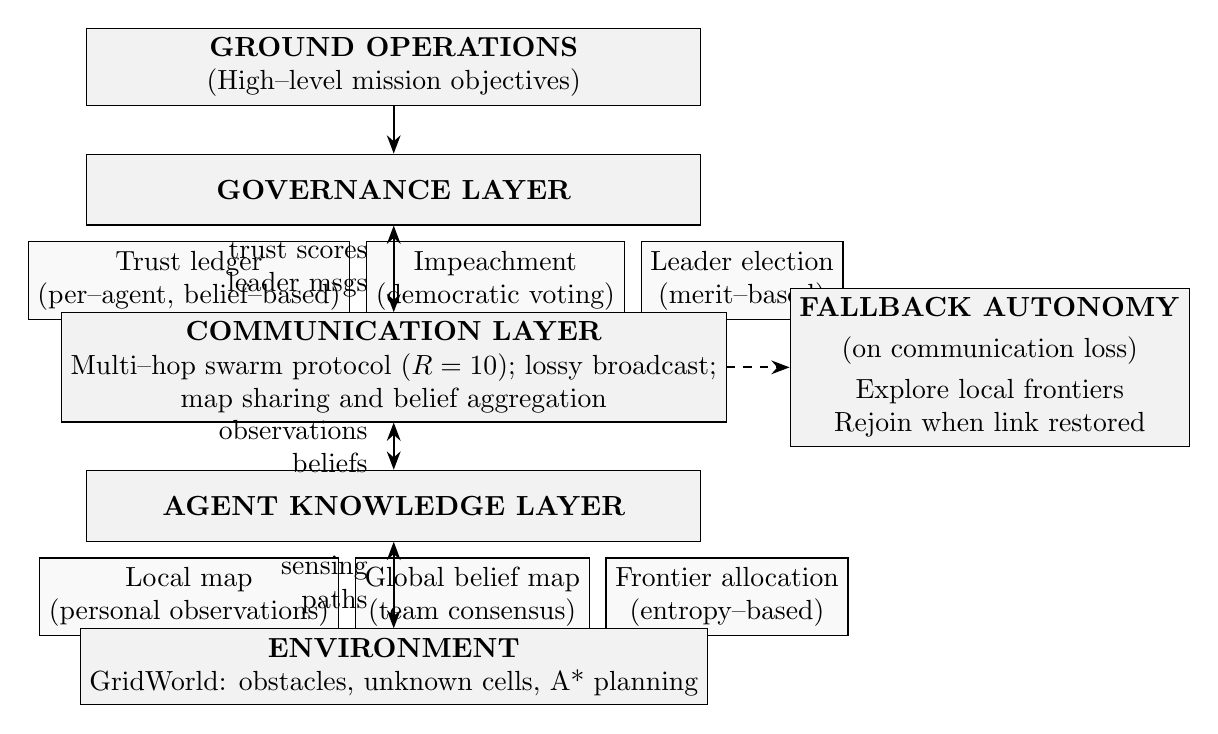
\begin{tikzpicture}[
    >=Stealth,
    layer/.style={
        draw,
        rectangle,
        minimum width=78mm,
        minimum height=9mm,
        align=center,
        fill=gray!10
    },
    subblock/.style={
        draw,
        rectangle,
        minimum width=24mm,
        minimum height=8mm,
        align=center,
        fill=gray!5
    },
    sideblock/.style={
        draw,
        rectangle,
        minimum width=28mm,
        minimum height=18mm,
        align=center,
        fill=gray!10
    },
    arrow/.style={-Stealth, thick},
    dblarrow/.style={Stealth-Stealth, thick},
    node distance=4mm
]

% Ground operations
\node[layer] (ground) {%
    \textbf{GROUND OPERATIONS}\\
    (High–level mission objectives)
};

% Governance layer
\node[layer, below=6mm of ground] (gov) {\textbf{GOVERNANCE LAYER}};

% Governance sub–blocks
\node[subblock, below=2mm of gov, xshift=-26mm] (trust) {%
    Trust ledger\\
    (per–agent, belief–based)
};
\node[subblock, right=2mm of trust] (impeach) {%
    Impeachment\\
    (democratic voting)
};
\node[subblock, right=2mm of impeach] (elect) {%
    Leader election\\
    (merit–based)
};

% Communication layer
\node[layer, below=11mm of gov] (comm) {%
    \textbf{COMMUNICATION LAYER}\\
    Multi–hop swarm protocol ($R=10$); lossy broadcast;\\
    map sharing and belief aggregation
};

% Knowledge layer
\node[layer, below=6mm of comm] (know) {\textbf{AGENT KNOWLEDGE LAYER}};

% Knowledge sub–blocks
\node[subblock, below=2mm of know, xshift=-26mm] (local) {%
    Local map\\
    (personal observations)
};
\node[subblock, right=2mm of local] (global) {%
    Global belief map\\
    (team consensus)
};
\node[subblock, right=2mm of global] (frontier) {%
    Frontier allocation\\
    (entropy–based)
};

% Environment
\node[layer, below=11mm of know] (env) {%
    \textbf{ENVIRONMENT}\\
    GridWorld: obstacles, unknown cells, A* planning
};

% Fallback autonomy (side block)
\node[sideblock, right=8mm of comm] (fallback) {%
    \textbf{FALLBACK AUTONOMY}\\[1mm]
    (on communication loss)\\[1mm]
    Explore local frontiers\\
    Rejoin when link restored
};

% Vertical data–flow arrows (labels moved to the LEFT of arrows)
\draw[arrow] (ground.south) -- (gov.north);

\draw[dblarrow] (gov.south) -- (comm.north)
  node[midway, left=2mm, align=right]{%
    trust scores\\leader msgs};

\draw[dblarrow] (comm.south) -- (know.north)
  node[midway, left=2mm, align=right]{%
    observations\\beliefs};

\draw[dblarrow] (know.south) -- (env.north)
  node[midway, left=2mm, align=right]{%
    sensing\\paths};

% Connection to fallback autonomy
\draw[arrow, dashed] (comm.east) -- (fallback.west);

\end{tikzpicture}%
}
\caption{REIP system architecture with governance, communication, and
agent-knowledge layers. Bidirectional arrows indicate data flow between
layers; fallback autonomy maintains exploration when agents lose
communication with the swarm.}
\label{fig:reip_arch}
\end{figure}



\end{document}